\section{Full state, basic and passivity-based feedback controllers} 
\label{sec:Full_state_feedback_controllers}

From the full dynamic model of the exoskeleton, a novel  full state feedback control law   was  derived and implemented. This control law is  identified in the following with the acronym JTFC1  and  explained in subsection \ref{subsec:JTFC1}.
To implement the control, the state of the system and, more in particular, the joint torque was estimated through a Kalman Filter described in  subsection \ref{subsec:kalmanTorque}.
To evaluate the performance of  the proposed full state feedback control,  two other torque controls inspired to existing joint torque controls available in literature have been implemented, identified respectively with the acronyms JTFC2 and JTFC3.
% We searched for torque controls designed for joint torque-based robots with a joint structure similar to the Rehab-Exos one.
\par The JTFC2, presented in subsection \ref{subsec:JTFC2}, is based on a  torque control   for  single joint based on torque sensor first  introduced by Hashimoto \cite{hashimoto1998experimental}. In order to compare the basic torque control with our full state feedback control, the Hashimoto formulation was extended and generalized to a multi-dof case. 
\par The JTFC3, reported in subsection \ref{subsec:JTFC3}, was inspired to the passivity-based control law \cite{kugi2008passivity}
implemented for the DLR Light Weight Robot III (LWR III)   that guarantees the passivity of the controlled system. The DLR LWR III shows a joint design compatible with the Rehab-Exos one, since both systems make use of the joint torque sensor to estimate the interaction torques/forces with the environment/human.


%%%%%%%%%%%%%%%%%%%%%%%%%%%%%%%%%%%%%%%%%%%%%%%%%%%%%%%%%%%%%%%%%%%%%%%%%%%%%%%%%%%%%%%%%%%%%%%%%%%%%%%%%%%%%%%%%%%%
%%%%%%%%%%%%%%%%%%%%%%%%%%%%%%%%%%%%%%%%%%%%%%%%%%%%%%%%%%%%%%%%%%%%%%%%%%%%%%%%%%%%%%%%%%%%%%%%%%%%%%%%%%%%%%%%%%%%
\subsection{An optimal observer for estimation of joint torque}\label{subsec:kalmanTorque}
Since the correct state estimation  is essential for the design of a full-state feedback joint-torque controller, the knowledge of the interaction torques between the human arm and the exoskeleton are required for  torque control implementation. The joint torque sensor provides a raw measurement $\tau_{s,i}$ that can be used together with the measured joint position $\theta_{m,i}$ to filter the sensed torque and to estimate the full system state, given by $[\tau_{s,i},\ \dot{\tau}_{s,i},\ \theta_{m,i},\ \dot{\theta}_{m,i},\ \tau_{d,i},\ \tau_{l,i}]$, where $\vects{\tau_l}=\vectm{J}^T \vects{F_l}$. 
Thus, a full-state Kalman filter has been designed to clean out both  $\theta_{m,i}$ from quantization noise $w_{\theta,i}$ and $\tau_{s,i}$ from measurement noise $w_{\tau,i}$, as well as to estimate the remaining variables.
%
\par 
Following \cite{vertechy2012interaction}, the dynamics of the two state components $\tau_{d,i}$ and $\tau_{l,i}$ can be modeled as two distinct Wiener processes (i.e. as two distinct non-stationary random processes) $\dot{\tau}_{d,i}=v_{d,i}$ and $\dot{\tau}_{l,i}=v_{l,i}$. Starting from equation (\ref{eq:dynamics_eq2}) the following meta-system can be derived:
%\ref{eq:dynamics_eq1},


%%%%%%DA VERIFICARE COSA SUCCESSO

\begin{equation}
\left \{
\begin{aligned}
\vects{\dot{\tau}_i} &=\vectm{A_i}\vects{\tau_i}+\vectm{B_i}\vects{\tau_{m,i}}+\vectmm{\Gamma}\vects{v_i} \\
		\vects{y_i} &=\vectm{C}\vects{\tau_i}+\vects{w_i}
		\end{aligned}
		\right .
		\label{eq:metasystem}
		\end{equation}
		%
		where $\vects{\tau_i}^T=[ \dot{\tau}_{s,i}\ \tau_{s,i}\ \dot{\theta}_{m,i}\ \theta_{m,i}\  \tau_{l,i} \tau_{d,i}\ ]$ is the meta-state vector, $\vects{v_i}^T=[ v_{l,i}\ v_{d,i} ]$ is the vector of process noises with variances $V_{l,i}$ and $V_{d,i}$, $\vects{w_i}^T=[ w_{\tau,i}\ w_{\theta,i} ]$ is the vector of measurement noises with variances $W_{l,i}$ and $W_{d,i}$, whereas:
		%
		\begin{equation}
		\begin{aligned}
		\vectm{A_i}=\mat{ \frac{-c_{t,i}}{J_i}  & \frac{-k_{t,i}}{J_i}& \frac{k_{t,i}b_{m,i}}{J_{m,i}} & 0 & \frac{ k_{t,i}}{J_{l,i}} &  \frac{-k_{t,i}}{J_{m,i}} \\
			1 & 0 & 0 & 0 & 0 & 0\\
			\frac{c_{t,i}}{  k_{t,i} J_{m,i} }&  \frac{1}{J_{m,i}} &  \frac{ -b_{m,i}}{J_{m,i}} & 0 & 0 &  \frac{1}{J_{m,i}}\\
			0 & 0 & 1 & 0 & 0 & 0\\
			0 & 0 & 0 & 0 & 0 & 0\\
			0 & 0 & 0 & 0 & 0 & 0} \\
		\vectm{B_i}=\vectlong{ \frac{ -k_{t,i}}{J_{m,i}} \\ 0 \\ \frac{1}{J_{m,i}} \\ 0 \\ 0 \\ 0}  \quad
		\vectmm{\Gamma}=\mat{ 0 & 0 \\ 0 & 0 \\ 0 & 0 \\ 0 & 0 \\ 1 & 0 \\ 0 & 1} \quad
		\vectm{C}=\mat{0 & 0 \\  1 & 0 \\  0 & 0  \\
			0 & 1 \\  0 & 0 \\ 0 & 0 } 
		\end{aligned}
		\label{stateobserver}
		\end{equation}
		%%%%%%%%%%%%%%%%%%%%%%%%%%%%%%%%%%%%%%%%%%%%%%%%%%%%%%%%%%%%%%%%%%%%%%%%%%%%%%%%%%%%%%%%%%%%%%%%%%%%%%%%%%%%%%%%%%%%
		%%%%%%%%%%%%%%%%%%%%%%%%%%%%%%%%%%%%%%%%%%%%%%%%%%%%%%%%%%%%%%%%%%%%%%%%%%%%%%%%%%%%%%%%%%%%%%%%%%%%%%%%%%%%%%%%%%%%


	\subsection{A full state feedback controller (JTFC1)} \label{subsec:JTFC1}
	
	The proposed control law is based on the full state obtained from the state  observer described by (\ref{eq:metasystem})  (\ref{stateobserver}), where the input control $\vect{u}$ is splitted up into one term $\vect{u_f}$, which implement control force behavior, and another term $\vects{u_g}$, which acts as a gravity compensation
	
	\begin{equation}
	\label{generic_control_law1}
	\begin{aligned}
	\vect{u} &= \vect{u_f} + \vect{u_g}
	\end{aligned}
	\end{equation}
	
The two above terms are expressed as:
	
	\setlength{\arraycolsep}{0.0em}
	
	\begin{eqnarray}{ll}
			\label{eq:JTCF1_control_law_uf_simple}
				\vect{u_g} &= \vect{G}(\vectm{D}\vects{\hat{\uptheta}_m}) \\
			\vect{u_f} &=  -\overbrace{\colorboxed{green}{\vectm{I^{-1}_i} \vectm{I_m} \vects{\uptau^D_s}}}^{\text{desired torque}}
			- \overbrace{\colorboxed{red}{\vectm{I_m} \vectm{K^{-1}_t} (\vects{\ddot{\uptau}_s^D}- \vectm{K_d} \vect{\dot{e}} -  \vectm{K_p} \vect{e}  )}}^{\text{state feedback}} + 	\nonumber \\
			&     +
			\underbrace{\colorboxed{blue}{ (\vectm{I_m} \overline{\vectm{M}^{-1}}  \vectm{J^T} \vects{\hat{F}_l}+ \vectm{B_m} \vectm{D}\vects{\dot{\uptheta}_m} {-}\:\vects{\hat{\uptau}_d} ) }}_{\text{unmodeled dynamics compensation}}
			\label{eq:JTCF1_control_law_b}
		\end{eqnarray}
			
%*****************************************
%
			

	\setlength{\arraycolsep}{5pt}
	
	where  $\vect{e}=\vects{\uptau_s}-\vects{\uptau_s^D}$ is the error on sensor torque, given the desired sensor torque  $\vects{\uptau_s^D}$.
	Let us assume moreover that
	
	\begin{equation}
 \left\{ \,
	\begin{IEEEeqnarraybox}[][c]{l?s}
	\IEEEstrut
\vects{\dot{\uptau}_s^D=0}  & so $\vect{\dot{e}}=\vects{\dot{\uptau}_s}$, \\
\vects{\ddot{\uptau}_s^D=0} & so $\vect{\ddot{e}}=\vects{\ddot{\uptau}_s}$. 
	\IEEEstrut
	\end{IEEEeqnarraybox}
	\right.
	\label{eq:conditions}
	\end{equation}




	
	The modified dynamics with the control laws  (\ref{generic_control_law1}), (\ref{eq:JTCF1_control_law_a}) and (\ref{eq:JTCF1_control_law_b}), leads to a stable error dynamics equations:
	
	\begin{equation}
%	\vects{\ddot{\uptheta}_m} &= \vectm{D}^{-1} (\vects{\ddot{\uptheta}} -\vectm{K_t^{-1}} \vect{\ddot{e}})
%\\
	\vects{0}  = \vect{\ddot{e}} + ( \vectm{C_t} \vectm{I_i^{-1}} + \vectm{K_d} )\vect{\dot{e}}+ ( \vectm{K_t} \vectm{I_i^{-1}}  + \vectm{K_p}   )\vect{e}
	\end{equation}
	
	The convergence of error $\vects{e}$ to zero can so be adjusted by choosing the proportional and derivative gains $\vectm{K_p}$ and $\vectm{K_d}$, to obtain the desired dynamic response.
	
	
	Based on the above, from the double derivation of \eqref{eq:taus}, we obtain the dynamics
	\begin{equation} 
	\vects{\ddot{\uptheta}_m} = \vectm{D}^{-1} (\vects{\ddot{\uptheta}} -\vectm{K_t^{-1}} \vect{\ddot{e}}) \label{eq:taus_deriv} 
	\end{equation}	
	
	
	\par Figure \ref{fig:full state} reports the schema of the proposed full state feedback control that takes into account the dynamic compensation contributes. Note that the torque sensor reads $\uptau_{s,i}$ and the commanded motor torques  $\uptau_{m,i}$ are net of the gravity compensation term $u_g$.
	
	\begin{figure}[]
		\centering
	%	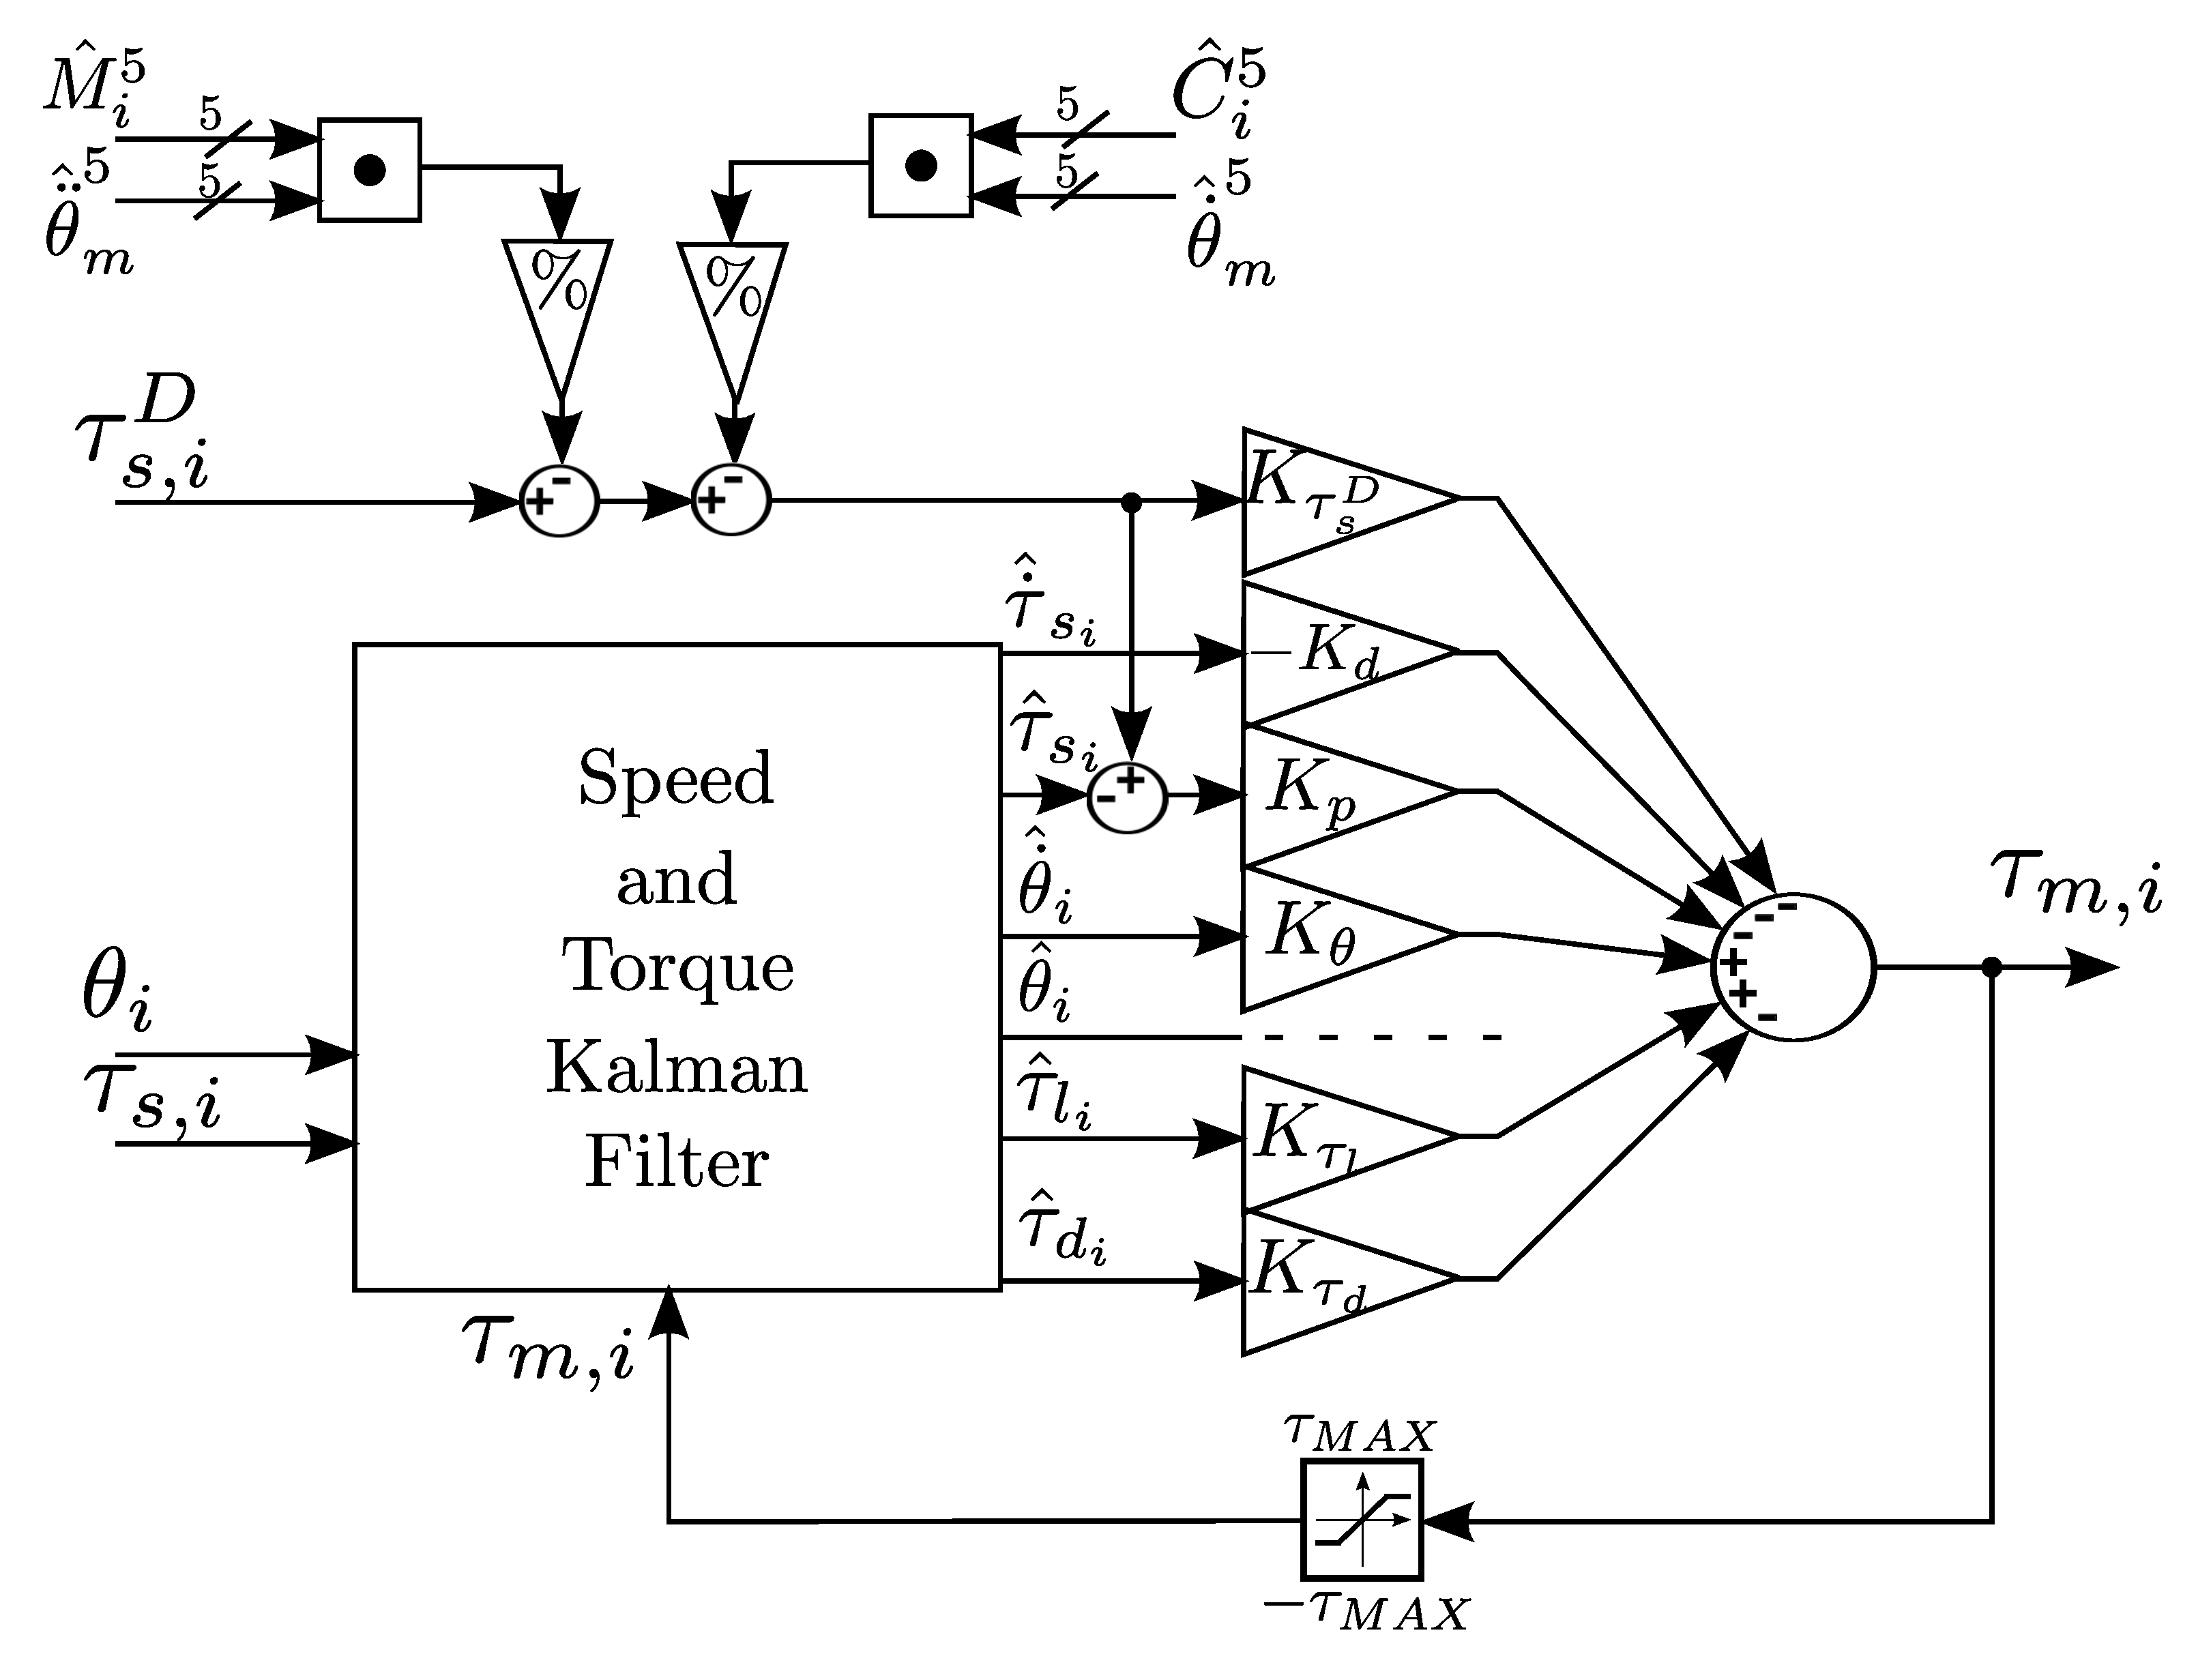
\includegraphics[width=1.0\columnwidth]{FullStateControlFeedback.pdf}
		\def\svgwidth{1\columnwidth}
		\begin{footnotesize}
			\input{imgRevised/feedbackController.pdf_tex}
		\end{footnotesize}
		\caption{The schema of the full state control feedback with the dynamic compensation.}
		\label{fig:fullstate}
	\end{figure}



%%%%%%%%%%%%%%%%%%%%%%%%%%%%%%%%%%%%%%%%%%%%%%%%%%%%%%%%%%%%%%%%%%%%%%%%%%%%%%%%%%%%%%%%%%%%%%%%%%%%%%%%%%%%%%%%%%%%
%%%%%%%%%%%%%%%%%%%%%%%%%%%%%%%%%%%%%%%%%%%%%%%%%%%%%%%%%%%%%%%%%%%%%%%%%%%%%%%%%%%%%%%%%%%%%%%%%%%%%%%%%%%%%%%%%%%%
\subsection{A basic state feedback controller (JTFC2)} \label{subsec:JTFC2}

The basic state feedback controller is derived assuming the following full model dynamics, extending the model introduced for a single joint by Hashimoto \cite{hashimoto1998experimental} where feedforward compensation using desired
torque is presented for  torque control using harmonic drive built-in torque sensor. The JTFC2 model  differs from (\ref{eqn:dinamicaLinkMultiGiunto})  since has no damping contribution of the elastic transmission and external forces.


The basic control law used in \cite{hashimoto1998experimental} can be generalized in case of multi-joint robot. Thus using the same notation and conditions of \eqref{eq:conditions}, the control law $\vects{u}_f$  can be written as a function of desired torque, where for $\vects{u}_g$ is used (\ref{eq:JTCF1_control_law_uf_simple}):




\setlength{\arraycolsep}{0.0em}
\begin{equation}
\label{JTFC2_control_law_final}
\vect{u_f} = - \underbrace{\colorboxed{green}{\vectm{I^{-1}_i} \vectm{I_m} \vects{\uptau^D_s}}}_{\text{desired torque}}
 - \underbrace{\colorboxed{red}{\vectm{I_m} \vectm{K^{-1}_t} (\vects{\ddot{\uptau}_s^D}- \vectm{K_d} \vect{\dot{e}} -  \vectm{K_p} \vect{e}  )}}_{\text{state feedback}}
\end{equation}
\setlength{\arraycolsep}{5pt}



The modified dynamics with the control law  (\ref{JTFC2_control_law_final}), leads to the following error dynamics equation:

\setlength{\arraycolsep}{0.0em}
\begin{IEEEeqnarraybox}[][c]{l}
%\label{JTFC2_error_equation1}
%\vects{\ddot{\uptheta}_m} &= \vectm{D^{-1}} \vects{\ddot{\uptheta}} - \vectm{D^{-1}} \vectm{K_t^{-1}} \vects{\ddot{e}}
%\\
\label{JTFC2_error_equation2}
\vectm{K_t}   \overline{\vectm{M}}^{-1}   \vectm{J^T} \vect{F_l} + \vectm{B_m D}\vects{\dot{\uptheta}_m}- \vectm{K_t} \vectm{I^{-1}_m} \vects{\uptau_d} \\= \vect{\ddot{e}} + (\vectm{K_d} + \vectm{I^{-1}_i} \vectm{C_t}) \vect{\dot{e}} + (\vectm{K_p} + \vectm{I^{-1}_i} \vectm{K_t}) \vect{e}
\end{IEEEeqnarraybox}
\setlength{\arraycolsep}{5pt}

%HOW IT SHOULD BE THE NEW EQUATION
%
%%%%%%%%%%%%%%%%%%%%%%%%%%%%%%%%%%%%%%%%%%%%%%%%%%%%%%%%%%%%%%%%%%%%%%%%%%%%%%%%%%%%%%%%%%%%%%%%%%%%%%%%%%%%%%%%%%%%
%%%%%%%%%%%%%%%%%%%%%%%%%%%%%%%%%%%%%%%%%%%%%%%%%%%%%%%%%%%%%%%%%%%%%%%%%%%%%%%%%%%%%%%%%%%%%%%%%%%%%%%%%%%%%%%%%%%%
\subsection{A passivity-based feedback controller (JTFC3)} \label{subsec:JTFC3}

The passivity-based state feedback is derived assuming the following full model dynamics (introduced by Ott in \cite{kugi2008passivity}), that differs from  (\ref{eqn:dinamicaLinkMultiGiunto}) for the absence of the motor's viscous friction term $\vectm{B_m } \vectm{D} \vects{\dot{\uptheta}_m} $. 
%and modeling of disturbance forces $\vects{\uptau_d} $:

%
%
%*********************************************

In \cite{kugi2008passivity} the control law $\vect{u}$ is designed as in (\ref{generic_control_law1}) where $\vect{u_g}$ are the torques due to the gravity, while %For this work $\vect{u_g}$ is calculated as in (\ref{eq:JTCF1_control_law_a}). 
the controller input $\vect{u_f}$  can optimize
the matching  with a desired impedance $\vectm{I}_{\theta}$, based on which the term $\vect{u_f}$ after some algebraic transformations can be written as:
%\hl{oppure una stima del tipo $\vects{G}(\vects{K^{-1}_t \uptau_s} - \vects{D \uptheta_m})$ OPPURE la loro}, while the term $\vects{u_f}$ is given by
%


\begin{equation}
\label{control_law_Kugi_2}
\vect{u_f} =  -  \underbrace{\colorboxed{green}{\vectm{I_m} \vectm{I^{-1}_{\uptheta}}  \vects{\uptau^D_s}}}_{\text{desired torque}}- 
 \underbrace{\colorboxed{red}{(\vectm{I}-\vectm{I_m} \vectm{I^{-1}_{\uptheta}}  )  (\vects{\uptau_s}+  \vectm{C_t}  \vectm{K_t}^{-1}\vects{\dot{\uptau}_s})  }}_{\text{state feedback}}
% \label{control_law_Kugi_3}
\end{equation}



So that the modified dynamics adopting the above control law  %(\ref{control_law_Kugi_2})
 leads to the following error dynamics equations where the error convergence can be set according to the selected value for $\vectm{I_{\uptheta}}$:

\setlength{\arraycolsep}{0.0em}

%%prova
%\footnotesize
\begin{equation}
\begin{IEEEeqnarraybox}[][c]{ll}
\label{JTFC3_error_equation_1}
%\vects{\ddot{\uptheta}_m} = \vectm{D^{-1}} \vects{\ddot{\uptheta}_j} - \vectm{D^{-1}} \vectm{K_t^{-1}} \vects{\ddot{e}}  
%\\
%\label{JTFC3_error_equation_2}
\vectm{K_t} \overline{\vectm{M}}^{-1}  \:(-\vects{\uptau_s^D} + \vectm{J^T} \vects{F_l}) +\\
%\vectm{K_t}   \overline{\vectm{M}}^{-1}   \vectm{J^T} \vect{F_l} 
+ \vectm{B_m D}\vects{\dot{\uptheta}_m}- \vectm{K_t} \vectm{I^{-1}_m} \vects{\uptau_d}= \nonumber \\
\vect{\ddot{e}} {+}\: \vectm{C_t} (  \vectm{I^{-1}_{\uptheta}} +  \vectm{\overline{M}^{-1}  } ) \vect{\dot{e}} 
{+}\: \vectm{K_t} (  \vectm{I^{-1}_{\uptheta}} +  \vectm{\overline{M}^{-1}  } ) \vect{e} 
\end{IEEEeqnarraybox}
\end{equation}
\setlength{\arraycolsep}{5pt}
\normalsize



%%%%%%%%%%%%%%%%%%%%%%%%%%%%%%%%%%%%%%%%%%%%%%%%%%%%%%%%%%%%%%%%%%%%%%%%%%%%%%%%%%%%%%%%%%%%%%%%%%%%%%%%%%%%%%%%%%%%
%%%%%%%%%%%%%%%%%%%%%%%%%%%%%%%%%%%%%%%%%%%%%%%%%%%%%%%%%%%%%%%%%%%%%%%%%%%%%%%%%%%%%%%%%%%%%%%%%%%%%%%%%%%%%%%%%%%%
\subsection{Haptic rendering} \label{sub:impedanceCJICF}

The three torque control laws are used as inner feedback loop of the impedance control used to test the exoskeleton in the haptic rendering task. The desired end-effector force $F_{ee}^D$ is due to the interaction with the virtual environment impedance. More in detail, the desired force is defined by:
%
\begin{equation}
\label{eq:desiredVE}
\left \{
\begin{aligned}
& \vect{ F_{ee}^D} = 0, \ \ \ \quad \quad \quad \quad \quad \quad \quad \quad  x < x_d \\
& \vect{F_{ee}^D} = \vectm{K_x} (\vects{x - x_d}) - \vectm{D_x}\vects{\dot{x}}, \quad  x \geq x_d  \\
\end{aligned}
\right .
\end{equation}
%
%\begin{equation}
%\tau^D = \vects{K_x} (\vects{x - x_d}) - \vects{D_x J \dot{\theta}} \frac{\vects{x - x_d}}{\left| \vects{x - x_d} \right|}
%\end{equation}
%
%obtaining the equivalent torque control law
%%
%\setlength{\arraycolsep}{0.0em}
%\begin{eqnarray}
%\label{eq:JICF1_control_law}
%\vects{u_f} = &&\: \vectm{B_m}  \vectm{D}\vects{\dot{\theta}_m} + \vectm{J_m} \vectm{\overline{M}^{-1}} \vectm{J^T} \vects{F_l} -\vects{\tau_d} \nonumber \\ 
%&&{-}\: {\vectm{J}_i^{-1}} \vectm{J_m J^T}(\vectm{K_x} (\vects{x - x_d}) - \vectm{D_x}\vects{\dot{x}}) \nonumber \\ 
%&&{+}\: \vectm{K_p} \vects{e} + \vectm{K_d} \vects{\dot{e}}
%\end{eqnarray}
%\setlength{\arraycolsep}{5pt}
%
where $\vect{x}$ is the coordinate along the normal axis to the surface, $\vect{x_d}$   is the wall coordinate, $\vectm{K_x}$ and $\vectm{D_x}$ are the desired stiffness and damping respectively of the simulated virtual environment.

%%%%%%%%%%%%%%%%%%%%%%%%%%%%%%%%%%%%%%%%%%%%%%%%%%%%%%%%%%%%%%%%%%%%%%%%%%%%%%%%%%%%%%%%%%%%%%%%%%%%%%%%%%%%%%%%%%%%
%%%%%%%%%%%%%%%%%%%%%%%%%%%%%%%%%%%%%%%%%%%%%%%%%%%%%%%%%%%%%%%%%%%%%%%%%%%%%%%%%%%%%%%%%%%%%%%%%%%%%%%%%%%%%%%%%%%%